% !TEX root = ../NeuralNetworksFR.tex

%%%%%%%%%%%%%%%%%%%%%%%%%%%%%%%%%%%%%%%%%%%%%%%%%%%%%%%%%%
%%%%%%%%%%%%%%%%%%%%%%%%%%%%%%%%%%%%%%%%%%%%%%%%%%%%%%%%%%
\section{L'algorithmique et les mathématiques de l'apprentissage}

Les réseaux de neurones sont des algorithmes, qui permettent à partir d'une entrée $\myblue{x}$ (par exemple une image) de calculer une sortie ${\color{red} y}$. Comme montré à la figure~\ref{fig:discriminative}, cette sortie est le plus souvent un ensemble de probabilités : par exemple la première sortie est la probabilité que l'image contienne un chat (plus ce nombre est proche de $100\%$, plus cela signifie que l'algorithme est sûr de lui), la deuxième est la probabilité que l'image contienne un chien, etc. 
%
Pour simplifier,  on ne considèrera dans nos exemples que deux classes : les chats et les chiens, mais en pratique on peut considérer une sortie  ${\color{red} y}$  avec plusieurs milliers de classes. On se restreint également à l'exemple des images, mais les réseaux de neurones sont également très performants pour reconnaitre des textes ou des vidéos.

Mathématiquement, un tel algorithme définit une fonction $f_{\mygreen{w}}$ (c'est-à-dire que ${\color{red} y} = f_{\mygreen{w}}({\color{blue}x})$). Le programme informatique qui permet de calculer cette fonction est très simple : il est composé d'un enchainement de plusieurs étapes, et chaque étape effectue des calculs élémentaires (des additions, des multiplications, et un maximum). 
%
En comparaison, les programmes informatiques que l'on trouve dans le système d'exploitation d'un ordinateur sont beaucoup plus complexes. 
%
Mais ce qui fait l'énorme différence entre un algorithme \guill{classique} et un réseau de neurones, c'est que ce dernier dépend de paramètres, qui sont les poids des neurones. Avant d'utiliser un réseau de neurones, il faut modifier ces poids pour que l'algorithme puisse résoudre le mieux possible la tâche demandée. Ceci s'effectue à l'aide de méthodes mathématiques et algorithmiques que l'on va expliquer dans les sections suivantes. C'est ce que l'on appelle \guill{entrainer} un réseau de neurone, et ceci nécessite beaucoup de temps, de calculs machine et d'énergie. 


Utiliser à bon escient de tels algorithmes nécessite donc des compétences en informatique et en mathématiques. Il faut ainsi manipuler les concepts clefs de l'algorithmique (méthodes itératives, temps de calcul, espace mémoire, implémentation efficace, \ldots) et des mathématiques (algèbre linéaire, optimisation, statistiques, \ldots).  

%%%%%%%%%%%%%%%%%%%%%%%%%%%%%%%%%%%%%%%%%%%%%%%%%%%%%%%%%%
\section{Réseaux de neurones discriminatifs}

Un réseau de neurones artificiel est construit autour d'une métaphore biologique. 
%
On connait relativement bien la structure du cortex visuel primaire, et la découverte en 1962 de l'organisation des neurones dans les premières couches~\cite{hubel1962receptive} a valu le prix Nobel en physiologie à Hubel et Wiesel. 
%
Ainsi, dans une vision extrêmement simplifiée du fonctionnement du cerveau, les neurones sont organisés en couches, chaque neurone récupère de l'information d'une couche précédente, effectue un calcul très simple, et communique son résultat à des neurones de la couche suivante. 
%
Il faut cependant garder à l'esprit qu'il ne s'agit que d'une métaphore et une source d'inspiration : les réseaux biologiques ont des connexions beaucoup plus complexes et les équations mathématiques qui les régissent sont également très complexes (elles ont été découvertes par Alan Hodgkin et Andrew Huxley en 1952~\cite{hodgkin1952quantitative} et ils ont eu le prix Nobel). 
%
Il reste ainsi difficile de mettre précisément en relation les performances parfois surprenantes des neurones artificiels et les capacités cognitives du cerveau. Par exemple, les techniques d'entrainement des réseaux artificiels que l'on va maintenant expliquer sont très différentes de la façon dont un enfant apprend.  

\begin{figure}\centering
	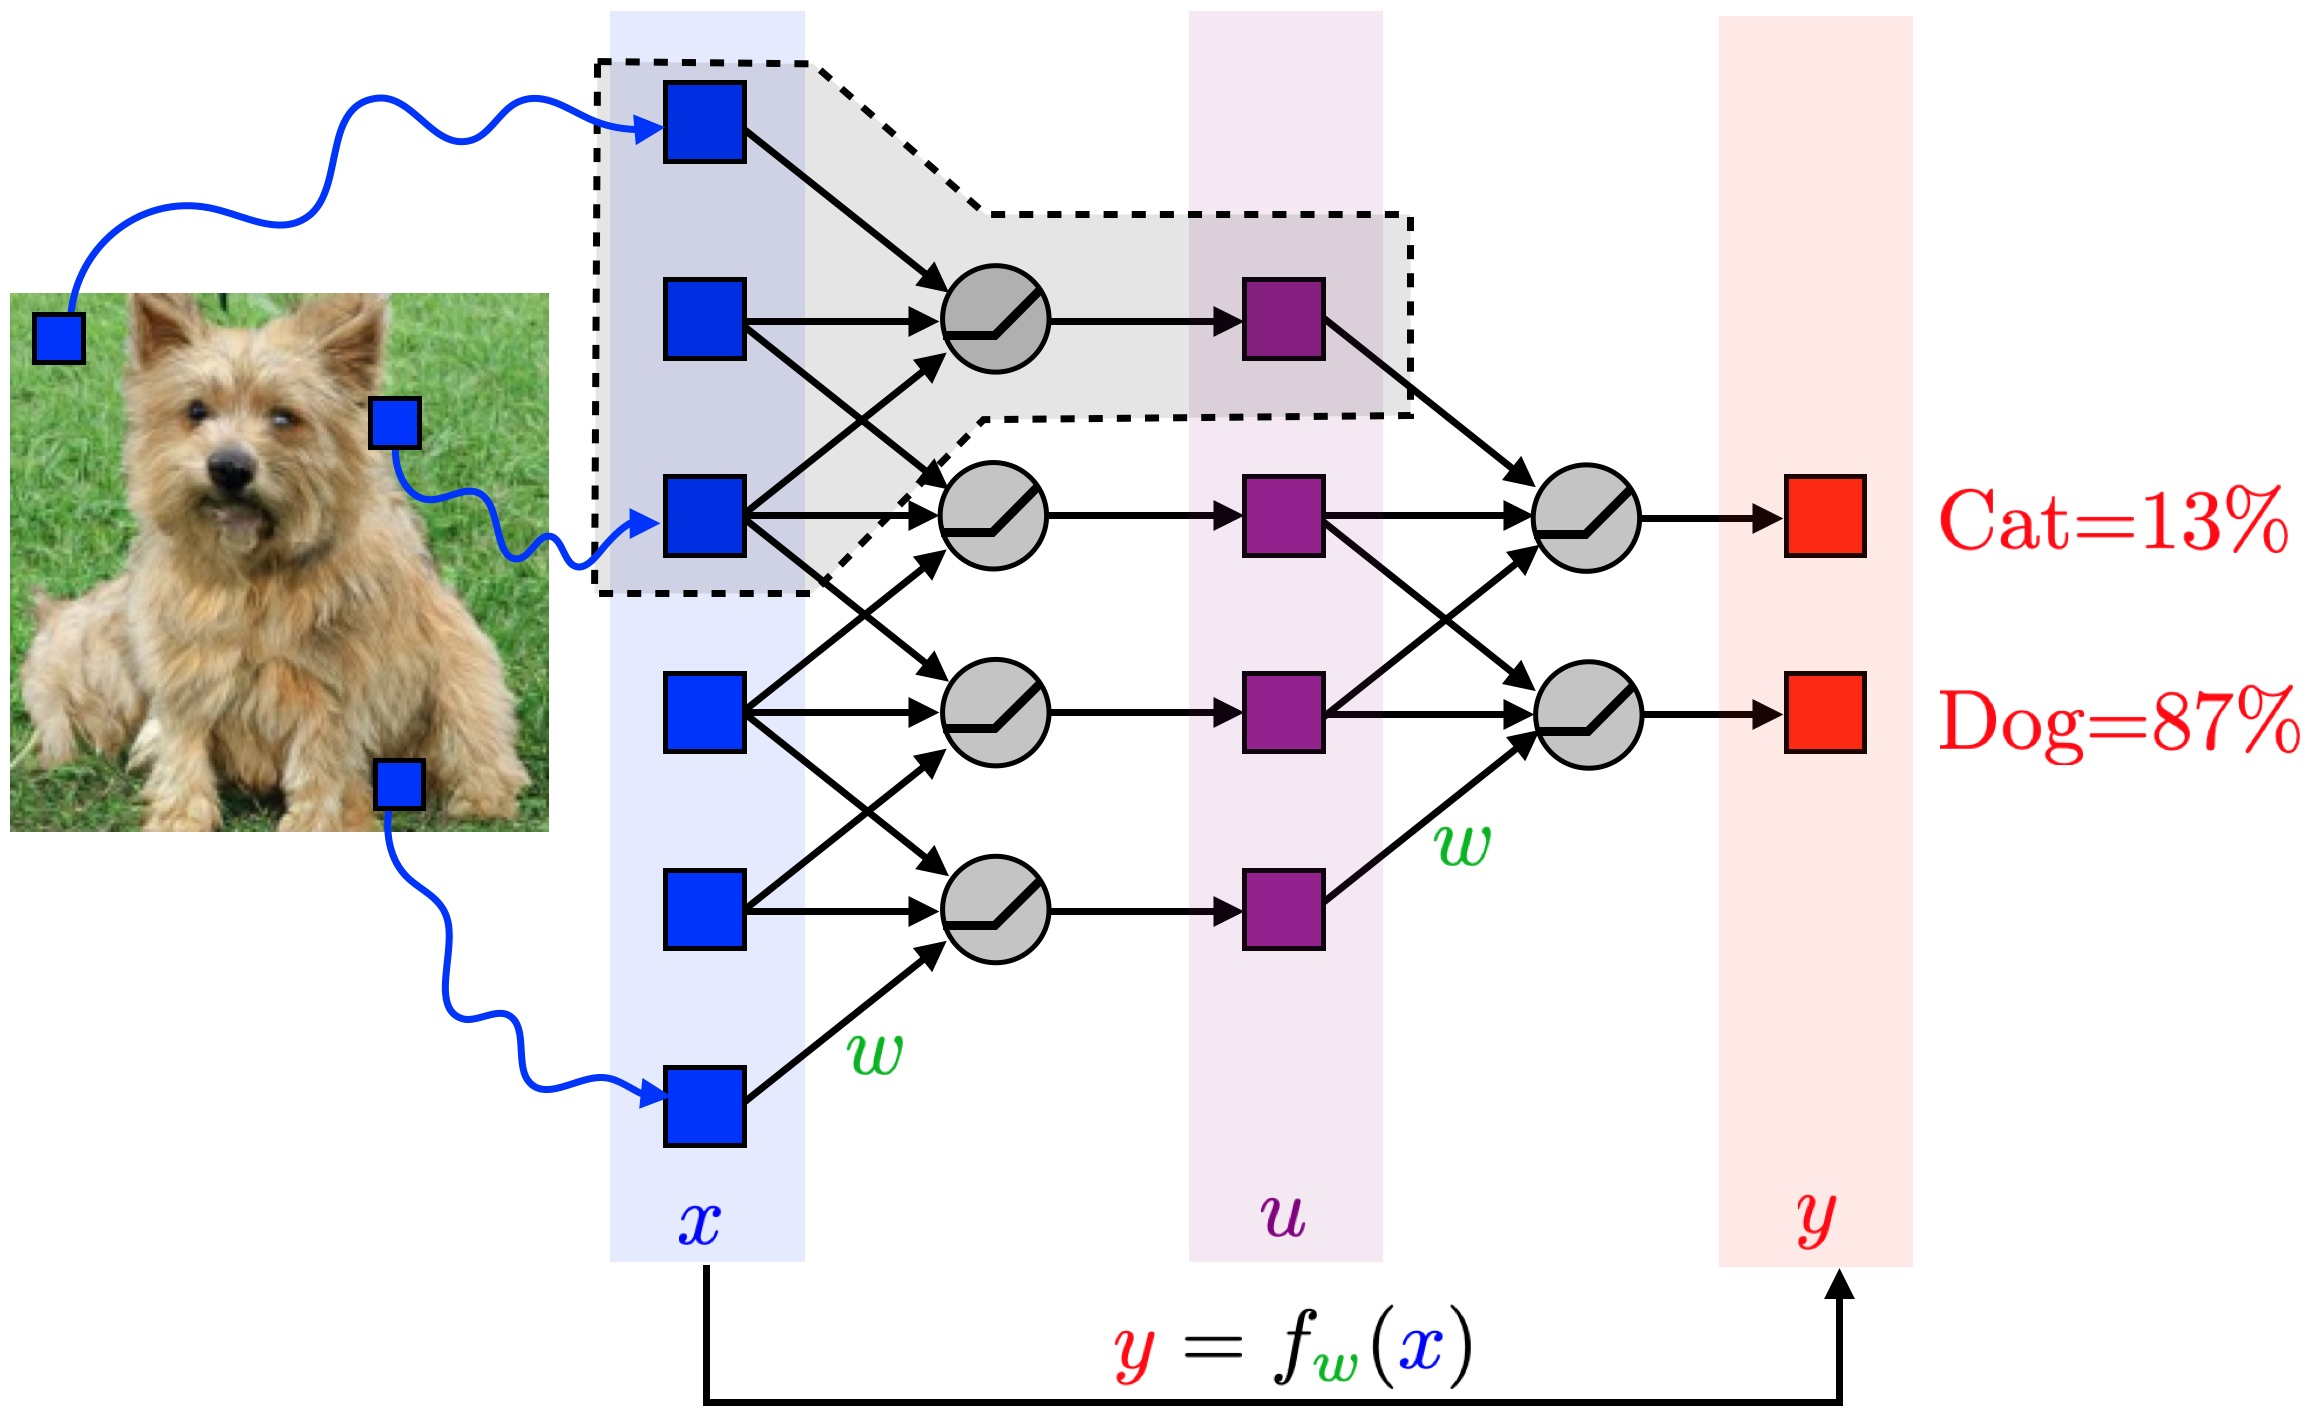
\includegraphics[width=.8\linewidth]{discriminative}
\caption{\label{fig:discriminative} Exemple d'un réseau de neurones discriminatif avec deux couches.  }
\end{figure}

La figure~\ref{fig:discriminative} détaille un exemple d'un tel réseau artificiel.
%
Ce type de neuron a été introduit en 1943 par McCulloch et Pitts~\cite{mcculloch1943logical}.
%
Pour simplifier, il est ici composé de seulement deux couches de neurones (la première couche entre ${\color{blue} x}$ et ${\color[rgb]{.5,0,.5} u}$, la deuxième entre ${\color[rgb]{.5,0,.5} u}$ et ${\color{red} y}$), mais les réseaux actuels les plus performants peuvent comporter plusieurs dizaines de couches, on dit qu'ils sont plus profonds. 
%
Dans notre exemple, les entrées ${\color{blue} x}$ sont les pixels d'une image. Une image contient typiquement des millions de pixels, et la figure n'en représente volontairement qu'un petit nombre : un réseau réaliste est très complexe. De plus, chaque pixel qui compose ${\color{blue} x}$ est en fait composé de 3 valeurs (une pour chaque couleur primaire rouge, vert et bleu). 

Le passage d'une couche (par exemple la couche ${\color{blue} x}$ des entrées) à une autre (par exemple la deuxième couche ${\color[rgb]{.5,0,.5} u}$, qui est une couche \guill{cachée} au milieu du réseau) se fait par l'intermédiaire d'un ensemble de neurones artificiels. Un neurone est représenté sur la figure~\ref{fig:neuron}. C'est le premier neurone, celui qui calcule la première valeur ${\color[rgb]{.5,0,.5} u_1}$ qui compose la couche ${\color[rgb]{.5,0,.5} u}$. Ce neurone connecte un certain nombre d'éléments de la première couche (ici trois : ${\color{blue} x_1, x_2, x_3}$, mais il peut y en avoir plus) à un seul élément de la deuxième, donc ici ${\color[rgb]{.5,0,.5} u_1}$. La formule calculée par le neurone est 
$$
	{\color[rgb]{.5,0,.5} u_1} = \max( \mygreen{w_1} \times \myblue{x_1} + \mygreen{w_2} \times \myblue{x_2} + \mygreen{w_3} \times \myblue{x_3} + \mygreen{w_4}, 0 ).
$$ 
Le neurone effectue ainsi une somme pondérée des trois entrées, avec trois poids $\mygreen{w_1},\mygreen{w_2},\mygreen{w_3}$, et on ajoute également $\mygreen{w_4}$, qui est un biais. Puis le neurone calcule le maximum entre cette somme et zero. On peut également utiliser une autre fonction que la fonction maximum, mais celle-ci est la plus populaire. Il s'agit d'une opération de seuillage. On peut la comparer aux neurones biologiques qui laissent ou non passer l'information suivant s'ils sont suffisamment excités ou pas.   
%
Ainsi, si la somme pondérée 
$\mygreen{w_1} {\color{blue} x_1} + \mygreen{w_2} {\color{blue} x_2} + \mygreen{w_3} {\color{blue} x_3} + \mygreen{w_4}$ 
est plus petite que 0, alors le neurone renvoie la valeur ${\color[rgb]{.5,0,.5} u_1}=0$, sinon il renvoie la valeur de cette somme et la place dans ${\color[rgb]{.5,0,.5} u_1}$.


\begin{figure}\centering
	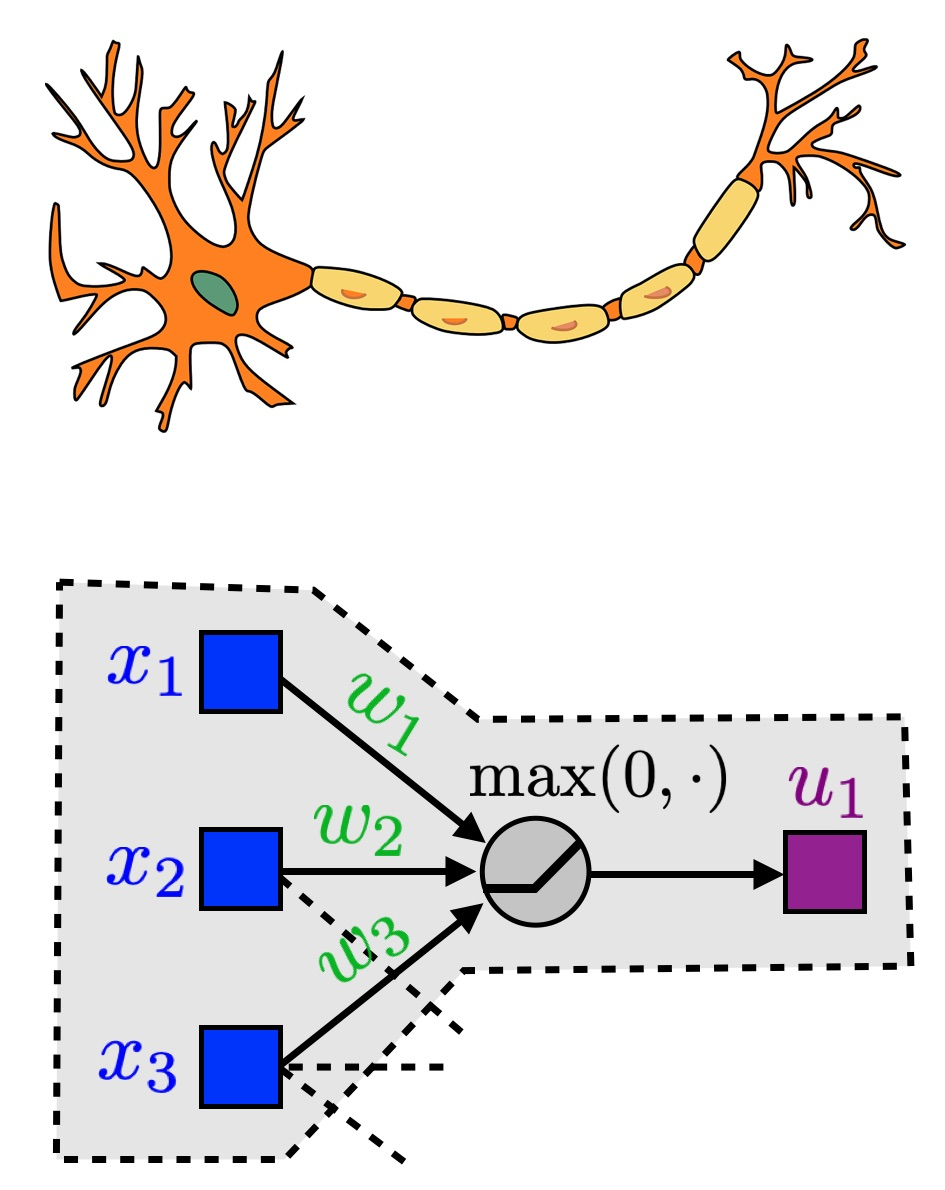
\includegraphics[width=.35\linewidth]{neuron}
\caption{\label{fig:neuron} Neurones biologique et artificiel. }
\end{figure}

De tels réseaux de neurones ont été introduits par Rosenblatt~\cite{rosenblatt1957perceptron} en 1957, qui les a appelés \guill{perceptrons}. 
% Ils ont ensuite été popularisés par le livre de Minsky et Papert~\cite{minsky1969perceptrons}. 
Les premiers perceptrons ne contenaient qu'une seule couche. 
%
De telles architectures avec une seule couche sont trop simples pour pouvoir effectuer des tâches complexes. C'est en rajoutant plusieurs couches que l'on peut calculer des fonctions plus complexes. 
%
Les réseaux de neurones profonds utilisent ainsi un très grand nombre de couches. Depuis quelques années, ces architectures ont permis d'obtenir des résultats très impressionnants pour faire de la reconnaissance d'images et de vidéos ainsi que pour la traduction automatique de textes. Ce sont ces recherches sur les réseaux profonds qui ont permises au chercheur français Yann Le Cun ainsi qu'à Geoffrey Hinton et Yoshua Bengio~\cite{lecun2015deep} d'obtenir le prix Turing en 2019. Ce prix est considéré comme étant l'équivalent du prix Nobel en informatique.  
%
Pour se familiariser avec ces réseaux multi-couches, on peut utiliser l'application interactive \url{https://playground.tensorflow.org}.

%%%%%%%%%%%%%%%%%%%%%%%%%%%%%%%%%%%%%%%%%%%%%%%%%%%%%%%%%%
\section{L'apprentissage supervisé d'un réseau de neurones}

L'entrainement d'un réseau de neurones consiste à choisir les \guill{meilleurs} poids possibles de l'ensemble des neurones qui compose un réseau (par exemple en particulier les poids $\mygreen{w_1, w_2}$ et $\mygreen{w_3}$ du neurone montré à la figure~\ref{fig:neuron}). 
%
Il faut ainsi choisir les valeurs de ces poids afin de résoudre le mieux possible la tâche étudiée, et ceci sur un ensemble de données d'apprentissage. 
%
Pour la reconnaissance d'objets dans les images, il s'agit d'un problème d'apprentissage supervisé : on dispose à la fois des images ${\color{blue} x}$ et des ${\color{red} y}$ (les probabilités de présence d'un chat et/ou d'un chien dans l'image).
%
La figure~\ref{fig:dataset} montre quelques exemples d'images utilisées pour entrainer un réseau, pour lesquelles on sait ce qu'elles contiennent (la classe des chats et la classe des chiens). 
%
Il faut donc, en amont de la phase d'apprentissage, que des humains fasse un long et fastidieux travail d'étiquetage de milliers voir de millions d'images. 


\begin{figure}\centering
	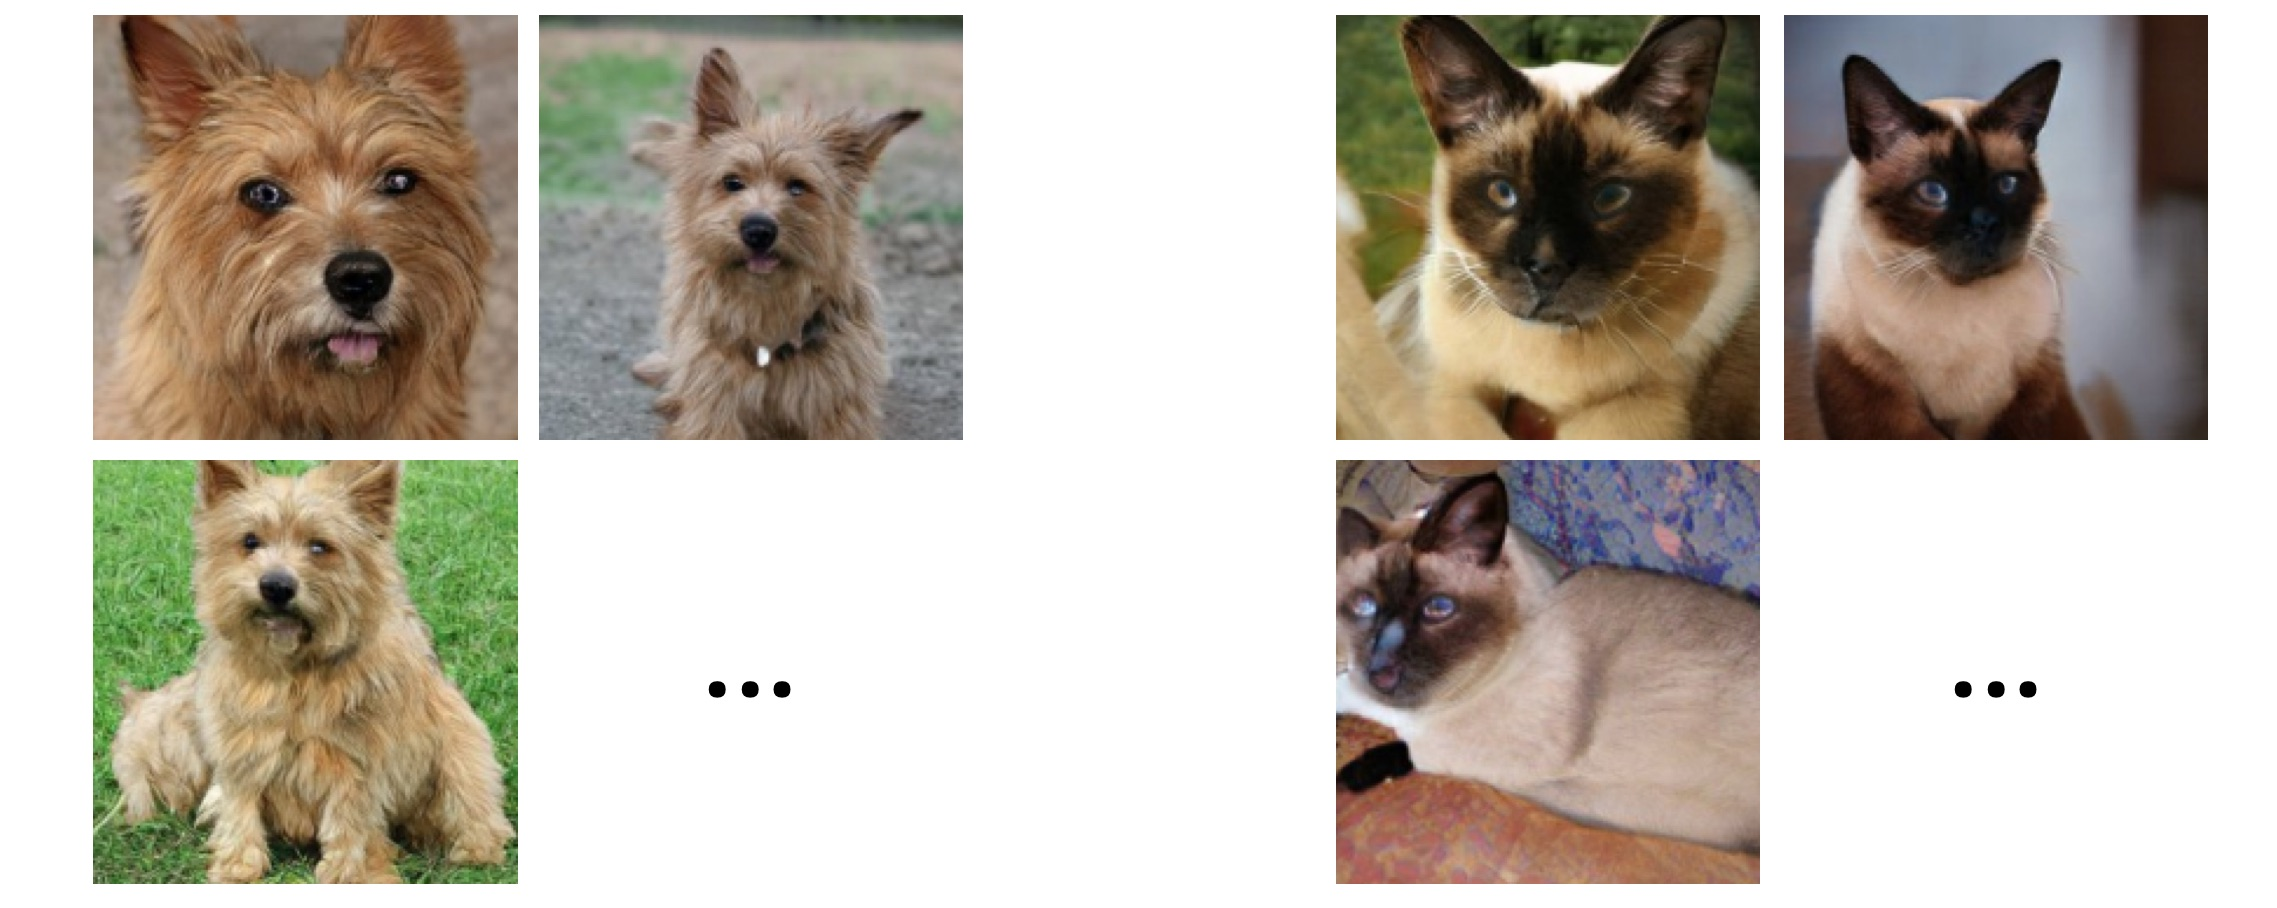
\includegraphics[width=.8\linewidth]{dataset}
\caption{\label{fig:dataset} Exemples d'images issues de la base de données ImageNet~\cite{deng2009imagenet} utilisées pour l'apprentissage. }
\end{figure}

La procédure d'entrainement consiste ainsi à modifier les poids $\mygreen{w}$ tels que pour chaque ${\color{blue}x}$, le réseau $f_{\mygreen{w}}$ prédise aussi précisément que possible le ${\color{red} y}$ associé, c'est-à-dire que l'on souhaite à la fin de l'entrainement que ${\color{red} y} \approx f_{\mygreen{w}}({\color{blue} x})$. 
%
Un choix simple est de minimiser la somme $E(\mygreen{w})$ des carrés des erreurs, ce qu'on écrit mathématiquement comme 
$$
	\min_{\mygreen{w}} E(\mygreen{w}) = \sum_{({\color{blue} x},{\color{red} y})} (f_{\mygreen{w}}({\color{blue} x}) - {\color{red} y})^2.
$$
%
Ceci correspond à un problème d'optimisation, car il faut trouver un jeu de paramètres qui optimise une certaine quantité d'intérêt. 
%
C'est un problème difficile, car il y a beaucoup de paramètres, et ces paramètres, surtout ceux des couches cachées, influencent de façon très subtile le résultat.
%
Heureusement, il existe des méthodes mathématiques et algorithmiques performantes pour résoudre de façon satisfaisante ce type de problème d'optimisation. Elles ne sont pas encore totalement comprises sur le plan théorique et c'est un domaine de recherche en pleine explosion.
%
Ces méthodes d'optimisation modifient les poids $\mygreen{w}$ du réseau pour l'améliorer et diminuer l'erreur d'entrainement $E(\mygreen{w})$. La règle mathématique pour décider de la stratégie de mise à jour des poids s'appelle la rétro-propagation~\cite{rumelhart1986learning} et est une merveille d'ingéniosité, c'est un cas particulier d'une méthode mathématique et algorithmique qui s'appelle la différentiation automatique à l'envers~\cite{linnainmaa1976taylor}.

Ces techniques d'apprentissage supervisé datent pour l'essentiel des année 1980. Mais c'est seulement en 2012 qu'un papier de Krizhevsky,  Sutskever et Hinton~\cite{krizhevsky2012imagenet} crée un coup de tonnerre en montrant que les réseaux profonds permettent de résoudre efficacement des problème de reconnaissance d'images. 
%
Cette révolution a été possible grâce à la combinaison de trois ingrédients: des nouvelles bases de données beaucoup plus grandes qu'auparavant~\cite{deng2009imagenet} ;  des grosses puissances de calcul grâce aux processeurs graphiques (les \guill{GPUs} , qui étaient auparavant cantonnés aux jeux vidéo) ;  l'introduction de plusieurs techniques d'optimisation qui stabilisent l'apprentissage~\cite{srivastava2014dropout}. 


%%%%%%%%%%%%%%%%%%%%%%%%%%%%%%%%%%%%%%%%%%%%%%%%%%%%%%%%%%
\section{L'efficacité des réseaux de neurones}

George Cybenko a démontré en 1989~\cite{cybenko1989approximation} qu'un réseau de neurones $f_{\mygreen{w}}$ avec deux couches peut approcher aussi précisément que l'on veut n'importe quelle fonction continue $f^\star$ (donc en quelque sorte résoudre n'importe quelle tâche, représentée par la fonction $f^\star$ inconnue, qui serait capable de reconnaitre des objets dans n'importe quelle image) pour peu que la taille de la couche interne ${\color[rgb]{.5,0,.5} u}$ (donc le nombre de neurones) soit arbitrairement grande.
%
Ce n'est pas pour autant qu'un tel réseau $f_{\mygreen{w}}$ avec seulement deux couches marche bien en pratique. Pour appliquer le théorème de Cybenko, il faut pouvoir disposer d'un nombre de donnée d'apprentissage potentiellement infini, ce qui est très loin d'être le cas en pratique.
%
Le but final de l'apprentissage n'est pas de minimiser l'erreur d'apprentissage $E(\mygreen{w})$, mais de pouvoir prédire aussi précisément que possible sur des nouvelles données. Si l'on dispose de peu de données, on risque de ne pas pouvoir apprendre assez précisément, et donc de faire des mauvaises prédictions : la fonction $f_{\mygreen{w}}$ sera en réalité très loin de la fonction $f^\star$ idéale que l'on voudrait apprendre si on avait une infinité d'exemples.  

Afin d'effectuer les meilleures prédictions possibles avec un nombre limité de données d'entrainement, on cherche donc les architectures de réseaux les plus adaptées, qui peuvent capter efficacement l'information présente dans les données. 
%
Les réseaux de neurones profonds (avec de nombreuses couches) mais avec relativement peu de connexions entre les couches se sont avérés très efficaces sur les données très \guill{structurées} comme les textes, les sons et les images. 
%
Par exemple, pour une image, les pixels ont des relations de voisinage, et on peut imposer des connexions spécifiques (une architecture) et ne pas connecter un neurone avec tous les autres mais seulement avec ses voisins (sinon il y aurait trop de connexions). De plus, on peut imposer que les poids associés à un neurone soit les mêmes que ceux associés à un autre neurone. On appelle ce type de réseaux les réseaux convolutifs~\cite{lecun1998gradient}. 
%
Pour l'instant, il n'y a pas d'analyse mathématique qui explique cette efficacité des réseaux convolutifs profonds. Il y a donc besoin de nouvelles avancées mathématiques pour comprendre les comportements et les limitations de ces réseaux profonds. 

